\section{Introduction}
\label{s:intro}
Due to the broadcast nature of wireless channels, there has been considerable attention to the security and privacy aspects of wireless communications. While the content of messages (i.e the information transmitted over the channel) can be protected against unauthorized access using cryptography or physical-layer security techniques \cite{zhou2013physical}, there are occasions when hiding the very existence of the communication channel is as vital as securing the communicated messages themselves. Examples of such situations are military operations, cyber-espionage, social unrest, or communication parties' privacy. All above have motivated the study of hidden communication channels, which are referred to as ``covert communication'' \cite{lampson1973note} in the literature.

There is a large body of work focusing on different schemes of covert communication applied into traditional wireless systems, but wireless systems research has expanded greatly in the past years to consider the potential impact of machine learning (ML) approaches for a variety of problems \cite{wang2017deep}. In fact, various network optimization problems, which were traditionally used to be handled with statistical models, are now leveraging machine learning techniques. Deep neural networks (DNNs) in particular, the major force in machine learning, have helped addressing several wireless problems, such as signal classification, channel estimation, transmitter identification, jamming and anti-jamming \cite{bahramali2021robust}. In a study conducted recently, as a replacement for conventional modular-based designs, an end-to-end communication model based on deep learning has emerged \cite{o2017introduction}. In this new paradigm, the transmitter and receiver are jointly trained as the encoder and decoder of an autoencoder network \cite{baldi2012autoencoders}. The autoencoder network can be trained to learn the characteristics of the signal, such as its statistical properties, and can then be used to perform compression or denoising on the signal. This improves the efficiency of the wireless transmission and helps to reduce the amount of errors that occur during the transmission. One noticeable difference between end-to-end systems and conventional modular designs is that in end-to-end systems, the encoder and decoder learn the coding and modulation tasks simultaneously as opposed to having separate modules for each. This gives autoencoder networks an advantage to enhance the error-correction capability of wireless systems by identifying and rectifying errors that happen during the transmission. Despite all these benefits, it has been established that deep learning models are highly susceptible to adversarial attacks \cite{bahramali2021robust, chakraborty2018adversarial}. This drives us to study the vulnerabilities that ML-based wireless communication systems might have against covert communications.

The preliminary attempt to obtain covertness started with the study of spread spectrum almost a century ago with the main purpose of hiding military communications \cite{scholtz1982origins}. The idea was to transmit the signal over a wide frequency band, which would make it harder to locate and identify the original signal amidst the background noise. Many works continued to further examine different aspects of this idea. However, the fundamental performance limits of such work were unknown until recently when Bash et al. \cite{bash2012square} established a square root limit on the number of covert bits that can be reliably sent over an additive white Gaussian noise (AWGN) channel. Following this work, there has been a surge of interest in examining covert channels \cite{sobers2017covert,soltani2018covert,sheikholeslami2018multi,cao2018wireless}.

Numerous works have studied the theoretical limits of covert communication over wireless systems in different scenarios \cite{bash2012square, soltani2018covert, sheikholeslami2018multi, li2021fundamental}, but only a few works have focused on practical implementation of covert communication. In almost all of these works, there is an external factor involved that the covert users relies on to build their covert communication. Some of which to mention are hardware impairments \cite{mohammed2021adversarial}, presence of a cooperative jammer \cite{sobers2017covert}, cooperation of a relay node \cite{liao2020generative, kim2022covert}. Beyond that, the majority of works make some favorable assumptions for covert users, such as existing a shared secret key between Alice and Bob unknown to Willie \cite{soltani2018covert}, accessibility of covert users to cover signals and modulation type \cite{grzesiak2021wireless}, uncertainty in the knowledge of noise power at Willie's receiver \cite{he2017covert}, neglecting the impact of the covert system on the normal communication \cite{mohammed2021adversarial}, and limiting the channel model to AWGN \cite{mohammed2021adversarial}. Imposing such restricted assumptions and dependencies eliminates the generality of these covert models and makes it difficult for them to adapt to different system deployments that have distinct conditions. Apart from that, recent studies indicate covert communication that causes noticeable divergence in the statistical properties of signals can be easily detected using analytical and steganalysis methods. \cite{bahramali2021robust,huang2020exploiting}.


\begin{figure}[tp!]
	\center
	\begin{subfigure}{0.45\textwidth}
		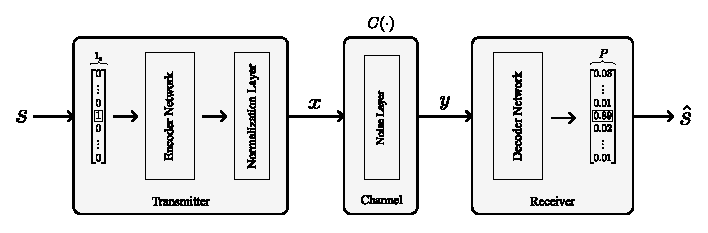
\includegraphics[width=\linewidth]{figs/original_autoencoder_architecture.eps}
	\end{subfigure}
	\\
	\caption{An end-to-end autoencoder-based communication system. The system takes a message \(s\) and outputs a probability distribution over all possible messages from which the most likely one is determined as the output \(\hat{s}\).}	
	\label{fig:original_autoencoder_architecture}
\end{figure}


In this work, we introduce a novel deep learning-based covert communication method that is free of many aforementioned assumptions. It merely relies on the existing channel's noise effect and is independent of any external factor. Our scheme also requires no knowledge of the cover signals, the modulation type, or even the channel type in single-user systems. We have optimized our solution to have the minimum impact on the normal communication while being stealth to a watchful system observer. More importantly, by training our covert models in an adversarial setting against the observer, we ensure our added covert signals make no conspicuous deviation in the statistical properties of signals. This prevents our covert signals to be easily detected using analytical tools. It is also worthwhile to mention that even though we are proposing our method for autoencoder-based wireless communication systems, there is no limitation on integrating our model into existing conventional wireless communication systems.


The contributions of this work can be expressed as follows:
\begin{enumerate}
	\item \textbf{Cover-Agnostic}: We propose a novel covert communication method using GANs that is independent of cover signals, waveforms, and modulation types of wireless systems.
	\item \textbf{Channel Independent}: In our proposed covert scheme, we train our model on three different channel models of AWGN, Rayleigh Fading, and Rician Fading and show our model does not rely on any information about the channel model nor the noise level.
	\item \textbf{Single-/Multi-User Adaptability}: We show that our work can be integrated both into single-user and multi-user communication setups and it is robust to channel interference. We also demonstrate there is a degree of freedom effect in our scheme, where increasing the number of users affects the performance of the covert and normal communication of the system in fading channels.
	\item \textbf{Undetectability}: By forming an adversarial competition between observer and covert users wherein one competes to outperform the other, we find an optimal solution that ensures observer of the system will perform almost no better than random guessing in differentiating the covert and non-covert transmissions.
	\item \textbf{Low Interference}: By evaluating the normal communication BLER after applying our covert model, we show that our covert scheme can be integrated into any normal communication system without having almost no disturbance on the ongoing normal communication.
\end{enumerate}
